\chapter{Ab initio exciton-phonon coupling}
\chaptertoc{}

\section{Introduction}
Mainly on monolayer, the three experiments
mention also the cathodoluminescence paper in which we see only the direct peak
say we did a benchmark on hBN
talk about the bBN and the reason we chose it : direct and indirect gaps are close in energy so we might see direct peak and phonon satellites. Indeed it was see experimentally so it is a good candidate for our method.\\
Chen Sangalli Bernardi.
cite Pedro Melo and say there is a different theoretical framework out of equilibrium, no need of steady-state. However, including the phonon-assisted transitions there is very challenging.\\
thus calculating the renormalization of the direct peak induced by the indirect transitions in the luminescence spectra.

\section{monolayer exciton dispersion}
fitting of the dispersion, Lbar vs Lfull
the nearly-free electron states at Gamma

\section{Theory of the ab initio exciton-phonon coupling}
In this section we present an \textit{ab initio} approach to obtain the exciton-phonon coupling matrix elements, that goes beyond the finite-difference approach presented in Sec. \ref{sec:excph_fdd}. The great advantage of this formulation is the possibility to integrate over exciton momenta in the full \acrlong{BZ} and to obtain the coupling of all excitons to all phonon modes.\\

For this work we based our numerical implementation on the formula derived by our collaborator Fulvio Paleari in his PhD thesis, \cite{paleari2019first} itself stemming from the theoretical work of Pierluigi Cudazzo published in Ref. \cite{cudazzo2020first}. In this approach, the electron-phonon interaction is included in the \acrshort{BSE} kernel via a phonon propagator. It induces a dynamic perturbation of the static electron-hole interaction contained in the kernel. It gives rise to a dynamical \acrlong{BSE}. Then, after a few approximations, the problem can be formally inverted and mapped onto an exciton-phonon Hamiltonian, which gives the exciton-phonon matrix elements. I refer the interested reader to these two references \cite{paleari2019first,cudazzo2020first}, where the rigorous derivation can be found.\\

In this thesis, I will present another way to derive the same exciton-phonon matrix elements, adapted from Ref. \cite{chen2020exciton}. It uses first-order perturbation theory for the excitonic Hamiltonian, the perturbation being a displacement of atoms along phonon modes. It introduces an additional interaction term due to the electron-phonon coupling, from which the exciton-phonon matrix elements can be identified. \\
Note that another, more general approach exists in litterature. It consists in treating the electron-electron, the electron-phonon interactions and the external field on the same footing,\cite{paleari2022exciton} which lifts some of the approximation we use, but it does not introduce relevant changes for the systems investigated here.\\

We consider a system with displacements from equilibrium positions $\boldsymbol{u}_{Ls}$ ($L$ labels the unit cell and $s$ the atom). We start from the \acrshort{DFT} level and take the Taylor expansion of the Kohn-Sham potential, labelled as $v_{\text{eff}}$ in Eq. \eqref{eq:KS_potential}, which we call $V^{KS}$ here. The expansion around the equilibrium positions reads :
\begin{equation}
    V^{KS}(\left\{ \uu_{Ls} \right\}) = V_0^{KS} + \sum_{Ls\alpha} \frac{\partial V^{KS}}{\partial \uu_{Ls\alpha}} \uu_{Ls\alpha} + \mathcal{O}(\left\{ \uu_{Ls} \right\}^2)
\end{equation}
The electronic wave functions and eigenvalues of the perturbed system depend on the atomic displacements $\left\{ \uu_{Ls} \right\}$. To obtain their change in the perturbed system, we apply first-order perturbation theory by keeping terms linear in $\left\{ \uu_{Ls} \right\}$. To first order, the correction to the eigenvalues vanishes while the correction to the Kohn-Sham wave functions $\psi_i$ (solutions of Eq. \eqref{eq:KS_eqs}) can be written as : 
\begin{equation}
    \delta\ket{\psi_i} = \sum_{j\neq i} \frac{\bra{\psi_j} \Delta V \ket{\psi_i}}{\epsilon_i - \epsilon_j} \ket{\psi_j}, \qquad \text{with} \ \ \Delta V = \sum_{Ls\alpha}\frac{\partial V^{KS}}{\partial \uu_{Ls}}\cdot \uu_{Ls}
\end{equation}
In the following, we use the tilde to label quantities of the perturbed system and write the perturbed wave function as :
\begin{equation}
    \ket{\tilde{\psi}_i} = \ket{\psi_i} + \delta\ket{\psi_i} = \ket{\psi_i} + \sum_{j \neq i} \Delta_{ij} \ket{\psi_j} \label{eq:perturb_wf}
\end{equation}
with
\begin{equation}
    \Delta_{ij} \equiv \frac{\bra{\psi_j} \Delta V \ket{\psi_i}}{\epsilon_i - \epsilon_j} \label{eq:Delta_var}
\end{equation}

We set ourselves in the Tamm-Dancoff approximation and we use the resonant Hamiltonian from Eq. \eqref{eq:H_BSE_res} as the  Hamiltonian of the unperturbed system $H \equiv H^{2p}(\{\boldsymbol{u}_{Ls} \}=0)$. For the perturbed system, we have $\Tilde{H} \equiv H^{2p}(\{\boldsymbol{u}_{Ls} \})$. 
The perturbed Hamiltonian matrix element is :
\begin{equation}
    \Tilde{H}_{\Tilde{v}\Tilde{c},\Tilde{v}'\Tilde{c}'}  = \bra{\Tilde{v}\Tilde{c}} \tilde{H} \ket{\Tilde{v}'\Tilde{c}'}  = ( \Tilde{\epsilon}_c - \Tilde{\epsilon}_v ) \delta_{\Tilde{v}\Tilde{v}'}\delta_{\Tilde{c}\Tilde{c}'} + \tilde{\Xi}_{\tv\tc}^{\tv'\tc'} \label{eq:perturbed_BSE}
\end{equation}
where $v,c$ refer to valence and conduction bands, respectively.
The perturbed Bethe-Salpeter kernel is defined just as in Eq. \eqref{eq:BSE_kernel_vc}, except that it is evaluated with the screened interaction of the perturbed system $\tilde{W}$, and its matrix elements are expressed in the perturbed basis.

Solving the \acrshort{BSE} in Eq. \eqref{eq:BSE_secular} gives the exciton wave functions that we will name $\ket{\lambda}$ and energies $E_{\lambda}$ :
\begin{align}
    \sum_{v',c'} H_{vc,v'c'} A_{\lambda}^{v'c'} &= E_{\lambda} A_{\lambda}^{vc} \\
    \ket{\lambda} = \sum_{vc}& A^{vc}_{\lambda}\ket{vc}
\end{align}
To derive the exciton-phonon interaction, we project the perturbed BSE Hamiltonian onto the unperturbed basis set and keep only the terms to first-order in the phonon perturbation. 
By such a process, the terms that will arise and be different from the unperturbed BSE Hamiltonian will define the exciton-phonon interaction.
One can show that to first order, the perturbed and unperturbed electronic energies coincide, so we will use $\Tilde{\epsilon}_i = \epsilon_i$. 
The perturbed Hamiltonian in the unperturbed basis is :
\begin{align*}
    \Tilde{H}_{\lambda\lambda'} = \bra{\lambda'} \Tilde{H} \ket{\lambda} &= \sum_{\Tilde{v}\Tilde{c},\Tilde{v}'\Tilde{c}'}  \bra{\lambda'}\ket{\Tilde{v}\Tilde{c}}\bra{\Tilde{v}\Tilde{c}} \Tilde{H} \ket{\Tilde{v}'\Tilde{c}'}\bra{\Tilde{v}'\Tilde{c}'}\ket{\lambda} \\
    &= \sum_{vc,v'c'}\sum_{\Tilde{v}\Tilde{c},\Tilde{v}'\Tilde{c}'} \bra{\lambda'}\ket{vc}\bra{vc}\ket{\Tilde{v}\Tilde{c}}\bra{\Tilde{v}\Tilde{c}} \Tilde{H} \ket{\Tilde{v}'\Tilde{c}'}\bra{\Tilde{v}'\Tilde{c}'}\ket{v'c'}\bra{v'c'}\ket{\lambda}
\end{align*}
where we used the completeness relations of both basis sets, $\sum_{vc}\ket{vc}\bra{vc} = \mathds{1}$ and $\sum_{\Tilde{v},\Tilde{c}} \ket{\Tilde{v}\Tilde{c}}\bra{\Tilde{v}\Tilde{c}} = \mathds{1}$. By definition of the BSE wave functions $\bra{v'c'}\ket{\lambda} = A_{\lambda}^{v'c'}$, then we can write the above equation as :
\begin{equation}
    \Tilde{H}_{\lambda\lambda'} = \bra{\lambda'} \Tilde{H} \ket{\lambda} = \sum_{vc,v'c'} A_{\lambda'}^{vc*} A_{\lambda}^{v'c'} \times \left[ \sum_{\Tilde{v}\Tilde{c},\Tilde{v}'\Tilde{c}'} \bra{vc}\ket{\Tilde{v}\Tilde{c}}  \bra{\Tilde{v}\Tilde{c}} \Tilde{H} \ket{\Tilde{v}'\Tilde{c}'} \bra{\Tilde{v}'\Tilde{c}'}\ket{v'c'} \right]
    \label{eq:exc_ham}
\end{equation}
The term inside the square brackets can be separated in two :
\begin{align*}
    &\sum_{\Tilde{v}\Tilde{c},\Tilde{v}'\Tilde{c}'} \bra{vc}\ket{\Tilde{v}\Tilde{c}}  \bra{\Tilde{v}\Tilde{c}} \Tilde{H} \ket{\Tilde{v}'\Tilde{c}'} \bra{\Tilde{v}'\Tilde{c}'}\ket{v'c'} =  \sum_{\Tilde{v}\Tilde{c},\Tilde{v}'\Tilde{c}'} \bra{vc}\ket{\Tilde{v}\Tilde{c}}  \left[ (\Tilde{\epsilon}_{\Tilde{c}} - \Tilde{\epsilon}_{\Tilde{v}}) \delta_{\Tilde{v}\Tilde{v}'}\delta_{\Tilde{c}\Tilde{c}'} + \tilde{\Xi}_{\tv\tc}^{\tv'\tc'} \right] \bra{\Tilde{v}'\Tilde{c}'}\ket{v'c'} \\
    &= \sum_{\Tilde{v}\Tilde{c}} \bra{vc}\ket{\Tilde{v}\Tilde{c}} (\epsilon_{\Tilde{c}} - \epsilon_{\Tilde{v}}) \bra{\Tilde{v}\Tilde{c}}\ket{v'c'} + \sum_{\Tilde{v}\Tilde{c},\Tilde{v}'\Tilde{c}'} \bra{vc}\ket{\Tilde{v}\Tilde{c}} \tilde{\Xi}_{\tv\tc}^{\tv'\tc'} \bra{\Tilde{v}'\Tilde{c}'}\ket{v'c'}
\end{align*}
We make the choice to approximate the perturbed kernel with the unperturbed one, $\tilde{\Xi}_{\tv\tc}^{\tv'\tc'} \approx \bra{\Tilde{v}\Tilde{c}} \Xi \ket{\Tilde{v}'\Tilde{c}'}$, that is to say the effect of atomic displacements on the screened interaction can be neglected and $W \approx \Tilde{W}$. This is the same approximation we took in Chapter 2 when we evaluated the response function by finite difference derivative. With this approximation we have :
\begin{equation}
    \sum_{\Tilde{v}\Tilde{c},\Tilde{v}'\Tilde{c}'} \bra{vc}\ket{\Tilde{v}\Tilde{c}} \tilde{\Xi}_{\tv\tc}^{\tv'\tc'} \bra{\Tilde{v}'\Tilde{c}'}\ket{v'c'} 
    \approx  \sum_{\Tilde{v}\Tilde{c},\Tilde{v}'\Tilde{c}'} \bra{vc}\ket{\Tilde{v}\Tilde{c}} 
    \bra{\Tilde{v}\Tilde{c}} \Xi \ket{\Tilde{v}'\Tilde{c}'}\bra{\Tilde{v}'\Tilde{c}'}\ket{v'c'} = \bra{vc} \Xi \ket{v'c'} = \Xi_{vc}^{v'c'}
\end{equation}
and thus the term in square brackets in Eq. \eqref{eq:exc_ham} becomes 
\begin{equation}
    \sum_{\Tilde{v}\Tilde{c},\Tilde{v}'\Tilde{c}'} \bra{vc}\ket{\Tilde{v}\Tilde{c}}  \bra{\Tilde{v}\Tilde{c}} \Tilde{H} \ket{\Tilde{v}'\Tilde{c}'} \bra{\Tilde{v}'\Tilde{c}'}\ket{v'c'} = \sum_{\Tilde{v}\Tilde{c}} \bra{vc}\ket{\Tilde{v}\Tilde{c}} (\epsilon_{\Tilde{v}} - \epsilon_{\Tilde{c}}) \bra{\Tilde{v}\Tilde{c}}\ket{v'c'} +  \Xi_{vc}^{v'c'} 
\end{equation}
Next, we use Eq. \eqref{eq:perturb_wf} to expand $\sum_{\Tilde{v}\tilde{c}} \bra{vc}\ket{\Tilde{v}\Tilde{c}} (\epsilon_{\Tilde{c}} - \epsilon_{\Tilde{v}})\bra{\Tilde{v}\Tilde{c}}\ket{v'c'}$ to order $\mathcal{O}(\Delta)$. We work within the Tamm-Dancoff approximation and keep only the resonant part of the BSE Hamiltonian; as a consequence, only valence-valence and conduction-conduction phonon-mediated scattering are allowed, that is to say $\Delta_{vc} = \Delta_{cv} = 0$ where the operator $\Delta$ was defined in Eq. \eqref{eq:Delta_var}. Using Eq. \eqref{eq:perturb_wf} we get :
\begin{align}
\begin{split}
    \bra{vc}\ket{\tv\tc} &= \bra{v}\ket{\tv}\bra{c}\ket{\tc} = \left(\delta_{v\tv} + \sum_{v''\neq\tv}\Delta_{\tv v''}\delta_{vv''}\right) \left(\delta_{c\tc} + \sum_{c''\neq \tc}\Delta_{\tc c''}\delta_{cc''}\right) \\
    &= \left( \delta_{v\tv}\delta_{c\tc} + \delta_{v\tv} \sum_{c''\neq\tc} \Delta_{\tc c''}\delta_{cc''} + \delta_{c\tc}\sum_{v''\neq \tv} \Delta_{\tv v''} \delta_{vv''} \right) + \mathcal{O}(\Delta^2)
\end{split}
\end{align}
and similarly
\begin{equation}
    \bra{\tv\tc}\ket{v'c'} = \bra{v'}\ket{\tv}^*\bra{c'}\ket{\tc}^* = \left( \delta_{v'\tv}\delta_{c'\tc} + \delta_{v'\tv} \sum_{c''\neq\tc} \Delta^*_{\tc c''}\delta_{c'c''} + \delta_{c'\tc}\sum_{v''\neq \tv} \Delta^*_{\tv v''} \delta_{v'v''}  \right)  + \mathcal{O}(\Delta^2)
\end{equation}
With these expressions, there are five first-order terms in $\sum_{\Tilde{v}\tilde{c}} \bra{vc}\ket{\Tilde{v}\Tilde{c}} (\epsilon_{\Tilde{c}} - \epsilon_{\Tilde{v}})\bra{\Tilde{v}\Tilde{c}}\ket{v'c'}$ that we can simplify using the Kronecker delta :
\begin{align}
    \sum_{\tv\tc} \bra{vc}\ket{\tv\tc} (\epsilon_{\Tilde{c}} - \epsilon_{\Tilde{v}})\bra{\tv\tc}\ket{v'c'} \nonumber \\
    %
        \approx (\epsilon_c - \epsilon_v)\delta_{vv'}\delta_{cc'} &+ \delta_{cc'}\sum_{\tv}(\epsilon_c - \epsilon_{\tv}) \sum_{v''\neq \tv} (\Delta^*_{\tv v''}\delta_{vv''}\delta_{v'\tv} + \Delta_{\tv v''}\delta_{v'v''}\delta_{v\tv}) \nonumber \\
        &+  \delta_{vv'} \sum_{\tc} (\epsilon_{\tc} - \epsilon_v) \sum_{c'' \neq\tc} (\Delta_{\tc c''}\delta_{cc''}\delta_{c'\tc} + \Delta^*_{\tc c''}\delta_{c'c''}\delta_{c\tc}) \nonumber \\
        %
        = (\epsilon_c - \epsilon_v)\delta_{vv'}\delta_{cc'} &+ \delta_{cc'} \left[  \sum_{v''\neq v'} (\epsilon_c - \epsilon_{v'}) \Delta^*_{v'v''}\delta_{v v''} + \sum_{v'' \neq v} (\epsilon_c - \epsilon_v) \Delta_{vv''} \delta_{v'v''} \right] \nonumber \\
        &+  \delta_{vv'} \left[ \sum_{c''\neq c'} (\epsilon_{c'} - \epsilon_v)\Delta_{c' c''}\delta_{cc''} + \sum_{c''\neq c} (\epsilon_c - \epsilon_v) \Delta^*_{cc''}\delta_{c'c''} \right] \nonumber \\
    %
    = (\epsilon_c - \epsilon_v) \delta_{vv'}\delta_{cc'} &+ \delta_{cc'}(\epsilon_{v'} - \epsilon_v) \Delta_{vv'} + \delta_{vv'}(\epsilon_c - \epsilon_{c'}) \Delta^*_{cc'}
\end{align}
where we used $\Delta_{ij} = -\Delta_{ji}^*$ to obtain the last line. Finally, the perturbed Hamiltonian in the excitonic basis in Eq. \eqref{eq:exc_ham} becomes :
\begin{align}
    \tilde{H}_{\lambda\lambda'} &= \sum_{vc,v'c'} A_{\lambda'}^{vc*} A_{\lambda}^{v'c'} \times \left\{ \left[ (\epsilon_c - \epsilon_v) \delta_{vv'}\delta_{cc'} + \Xi_{vc}^{v'c'} \right] + \delta_{cc'} (\epsilon_{v'} - \epsilon_v)\Delta_{vv'} + \delta_{vv'}(\epsilon_c - \epsilon_{c'}) \Delta_{cc'}^*  \right\} \nonumber \\
    &= E_{\lambda'}\delta_{\lambda\lambda'} + \sum_{vc,v'c'} A_{\lambda'}^{vc*} A_{\lambda}^{v'c'} \cdot \left( \delta_{cc'}(\epsilon_{v'} - \epsilon_v) \Delta_{vv'}  + \delta_{vv'} (\epsilon_c - \epsilon_{c'}) \Delta^*_{cc'} \right) \label{eq:perturb_H_exc}
\end{align}
where we use the fact that the unperturbed Hamiltonian is diagonalized by the Tamm-Dancoff exciton eigenvectors :
\begin{equation}
    E_{\lambda'}\delta_{\lambda\lambda'} = \sum_{vc,v'c'} A_{\lambda'}^{vc*} A_{\lambda}^{v'c'} \times \left( (\epsilon_c - \epsilon_v)\delta_{vv'}\delta_{cc'} + \Xi_{vc}^{v'c'} \right).
\end{equation}
Therefore, the first term in the second line of Eq. \eqref{eq:perturb_H_exc} is the unperturbed Hamiltonian, while the second term is the exciton-phonon interaction,
\begin{equation}
    \tilde{H}_{\text{exc-ph}} = \sum_{vc,v'c'} A_{\lambda'}^{vc*} A_{\lambda}^{v'c'} \cdot \left( \delta_{cc'}(\epsilon_{v'} - \epsilon_v) \Delta_{vv'}  + \delta_{vv'} (\epsilon_c - \epsilon_{c'}) \Delta^*_{cc'} \right). \label{eq:H_exc-ph}
\end{equation}
To obtain the final result, we reintroduce the periodicity of the Kohn-Sham states stemming from Bloch theorem :
\begin{equation}
    \ket{\phi_i} \to \ket{\phi_{n\kk}}
\end{equation}
and the transition basis set for an exciton with center of mass momentum $\QQ$ is $\ket{vc} = \ket{v\kk_v,c\kk_c} = \ket{v\kk_v,c\kk_v + \QQ}$. We write the change in potential due to atomic displacements in second quantization using the phonon normal coordinates :
\begin{equation}
    \Delta V = \sum_{\mu \qq} \sqrt{\frac{1}{2\Omega_{\mu\qq}}} \partial_{\mu\qq} V^{KS}(\hat{b}_{\mu\qq} + \hat{b}^\dagger_{\mu-\qq})  
\end{equation}
where the operator $\partial_{\mu\qq}$ should be understood as the derivative with respect to a displacement $R_{\mu\qq}$ along a phonon mode $\mu$ at momentum $\qq$. Then the $\Delta_{ij}$ describing the transition from $i$-th to $j$-th state becomes :
\begin{equation}
    \Delta_{n\kk n'\kk'} = \frac{\bra{n'\kk'} \Delta V \ket{n\kk}}{\epsilon_{n\kk} - \epsilon_{n'\kk'}} = \sum_{\mu\qq} \frac{g_{nn'\mu}(\kk,\qq) \delta(\kk'-\kk-\qq)}{\epsilon_{n\kk} - \epsilon_{n'\kk'}} (\hat{b}_{\mu\qq} + \hat{b}^\dagger_{\mu-\qq})
\end{equation}
where $g_{nn'\mu}(\kk,\qq)$ are the electron-phonon matrix elements defined in Eq. \eqref{eq:gkkp}, namely the probability amplitude for an electron in band $n$ with crystal momentum $\kk$ to transition to a final state in band $n'$ and momentum $\kk' = \kk+\qq$ by absorbing or emitting a phonon with mode index $\mu$ and wave vector $\qq$. The slight difference with Eq. \eqref{eq:gkkp} is that we change the arguments to have a more compact form : the first argument is the momentum of the initial state and the second argument is the phonon momentum.

To proceed, we have to make the approximation that the excitons are boson-like particles bound by the Coulomb interaction. We can then define a bosonic Hamiltonian for excitons :
\begin{equation}
    H_{\text{exc}} = \sum_\lambda E_\lambda (\QQ) \hat{a}^\dagger_{\lambda\QQ} \hat{a}_{\lambda\QQ}
\end{equation}
where $\hat{a}^\dagger_{\lambda\QQ}, \hat{a}_{\lambda\QQ}$ are the creation/annihilation operators for an exciton $\lambda$ with center-of-mass momentum $\QQ$ and energy $E_\lambda(\QQ)$. This is an approximation that ignores the fact that excitons are a pair of two bound fermions, this is why it works best at low exciton density so that the exciton are weakly interacting. It has been shown to correctly reproduce several experimental results.\cite{paleari2019exciton,perebeinos2005effect} However, there are theoretical evidence that the fermionic character of excitons cannot always be neglected.\cite{katzer2023excitonphononscattering}\\
Using this approximation we rewrite the exciton-phonon interaction from Eq. \eqref{eq:H_exc-ph} in second quantization :
\begin{equation}
    \tilde{H}_{\text{exc-ph}} = \sum_{\lambda\lambda'\mu, \QQ\qq} \mathcal{G}_{\lambda\lambda'}^{\mu}(\QQ,\qq) \hat{a}^\dagger_{\lambda\QQ+\qq} \hat{a}_{\lambda'\QQ} (\hat{b}_{\mu\qq} + \hat{b}^\dagger_{\mu-\qq}). \label{eq:H_excph}
\end{equation}
where we defined the exciton-phonon matrix elements as :
\begin{multline}
    \mathcal{G}_{\lambda\lambda'}^{\mu}(\QQ,\qq) = \sum_{\substack{vcv'c'\\ \kk_v \kk_c \kk'_{v'} \kk'_{c'}}} A_{\lambda\QQ+\qq}(v\kk_v,c\kk_c) A_{\lambda'\QQ}^*(v'\kk'_{v'},c'\kk'_{c'}) \\ 
    \times \left[ \delta_{vv'} g_{c'c\mu}(\kk'_{c'},\qq) \delta(\kk_c - \kk'_{c'} - \qq) \right. \left. - \delta_{cc'}g_{vv'\mu}(\kk_v,\qq) \delta(\kk'_{v'} - \kk_v -\qq) \right]. \label{eq:Gkkp_full}
\end{multline}
Let us make momentum conservation explicit to obtain the final expression. The exciton-phonon coupling constant $\mathcal{G}_{\lambda\lambda'\mu}(\QQ,\qq)$ is the probability amplitude for scattering from an exciton with band index $\lambda$ with center-of-mass momentum $\QQ + \qq$ to an exciton with band index $\lambda'$ and center-of-mass momentum $\QQ$. This convention will be clarified later. Since $A_{\lambda\QQ}(v\kk_{v},c\kk_{c}) \neq 0$ only for $\kk_c - \kk_v = \QQ$, in Eq. \eqref{eq:Gkkp_full} we can impose three constraints : $\kk_c - \kk_v = \QQ$, $\kk'_c - \kk'_v =\QQ + \qq$ and $\kk'_c - \kk_c = \qq$ (or $\kk'_v - \kk_v = \qq$). As a consequence, we drop three $\kk$-point \acrshort{BZ} summations and the final result for the exciton-phonon matrix element for a given exciton momentum $\QQ$ and phonon momentum $\qq$ is :
\begin{multline}
    \mathcal{G}_{\lambda\lambda'}^{\mu}(\QQ,\qq) \\
    = \sum_{\kk} \left[ \sum_{vcc'} A_{\lambda\QQ+\qq}(v\kk,c\kk+\QQ+\qq) A_{\lambda'\QQ}^{*}(v\kk,c'\kk+\QQ)g_{c'c\mu}(\kk+\QQ +\qq,-\qq) \right.\\
     \left. - \sum_{cvv'} A_{\lambda\QQ+\qq}(v\kk-\qq,c\kk+\QQ) A_{\lambda'\QQ}^*(v'\kk,c\kk+\QQ) g_{vv'\mu}(\kk-\qq,\qq) \right]. \label{eq:Gkkp}
\end{multline}
This is the general expression which was implemented in the \yambo~code. This expression is made of two contributions relative to the coupling of phonons with either the electron in the conduction band or the hole in the valence band constituting the exciton. It corresponds to a rotation of the electron-phonon coupling in the exciton basis. This basis shifts the picture from electrons and holes scattering with phonons to transitions between excitonic states mediated by phonons.

This formula allows to compute various quantities depending on the exciton-phonon matrix elements, such as the exciton lifetimes or more interestingly for us, the response function that includes phonon-assisted transitions. This will allow us to compute luminescence spectra. 

\section{Phonon-assisted response function}
Now we can proceed to the solution of the exciton-phonon Hamiltonian. A direct diagonalization is out of reach because the transitions at different $\QQ$ are mixed by the electron-phonon scattering, therefore the dimension of the Hilbert space becomes too large. Hence we will make use of \acrshort{MBPT} to find an approximate solution to Eq. \eqref{eq:H_excph}. The dynamical perturbation induced by the electron-phonon coupling adds a term to the \acrshort{BSE} kernel and it yields a general \textit{dynamical} \acrlong{BSE} :
\begin{equation}
    \mathcal{L}(1234) = L(1234) + \int d5678 \ L(1625) \ \tilde{\Xi}^{D}(5867) \ \mathcal{L}(7483) \label{eq:dBSE}
\end{equation}
where $L$ is the two-particle propagator solution of the static \acrshort{BSE} in Eq. \eqref{eq:BSE} and the kernel $\tilde{\Xi}^{D}$ has an additional dynamical term induced by the electron-phonon interaction. The dynamical kernel does not allow a direct inversion of the dynamical \acrshort{BSE} since it depends self-consistently on $L$ and cannot be written in terms of two times. We chose an approach that consists in taking the electron-phonon interaction only up to first order. This way, we define $L^{(1)}$ as the solution of Eq. \eqref{eq:dBSE}, obtained by replacing $\mathcal{L}$ on the right hand side of Eq. \ref{eq:dBSE} by the static $L$ :
\begin{equation}
    L^{(1)}(1234) = L(1234) + \int d5678 \ L(1625) \ \tilde{\Xi}(5867) \ L(7483)
\end{equation}
where $\Tilde{\Xi}$ is the kernel perturbed by first-order electron-phonon interaction, the same introduced in the above section in Eq. \eqref{eq:perturbed_BSE}. With this equation can consider only interaction mediated with a single phonon. Extension to multiple-phonon scattering exists in literature,\cite{perebeinos2008phonon} but the present formulation is the first order of a cumulant expansion and its generalization to coupling with phonons at all orders is straightforward.\cite{cudazzo2020first}\\
Using the relation Eq. \eqref{eq:chi_iL}, we can obtain the response function in the excitonic basis in terms of one frequency (or two times), including the first-order correction due to exciton-phonon coupling :
\begin{equation}
    \chi^{(1)}_{\lambda\lambda'}(\omega) = \chi_{\lambda\lambda'}(\omega) + \chi_{\lambda}(\omega) \ \Pi^{\text{excp-ph}}_{\lambda\lambda'} (\omega) \ \chi_{\lambda'}(\omega) \label{eq:chi_1}
\end{equation}
where we used the short-hand notation $\chi_{\lambda}(\omega) = \chi_{\lambda\lambda'} (\omega) \delta_{\lambda\lambda'}$. On the right hand side, the quantity $\Pi^{\text{excp-ph}}_{\lambda\lambda'} (\omega)$ is the exciton self-energy describing dynamical effects induced by the electron-phonon interaction. We will refer to it as \textit{exciton-phonon self-energy}. It can be computed explicitly in \acrshort{MBPT}\cite{mahan2000many} from the perturbed kernel $\tilde{\Xi}$ in the Tamm-Dancoff approximation, and we do it in a similar way as in Ref. \cite{giustino2017review} for the electron-phonon case. Owing to the fact that we consider the first order only in exciton-phonon scattering, we will have a self-energy similar to the Fan-Migdal one for the electron-phonon problem : $\Pi^{\text{excp-ph}} = \mathcal{G}^2DL$ where the exciton propagator $L$ replaces the electron one, $D$ is the phonon propagator and $\mathcal{G}$ are the exciton-phonon matrix elements derived in the previous section given by Eq. \eqref{eq:Gkkp}. 

Keeping only the first order dynamical correction allows scattering with only one phonon, but the use of a self-energy allows to formally write two different ways of summing contributions to infinite orders, hence scattering with any number of phonons. The first one is to take a Dyson equation $\chi^{D} = \chi + \chi \Pi^{\text{excp-ph}} \chi$ which corresponds to a partial re-summation of the general Eq. \eqref{eq:dBSE}.\cite{marini2003dynamical} It will yield the correction to the exciton energies due to coupling with phonons but will fail to describe the phonon satellites in the optical spectra, just as the \acrshort{PES} satellites given by the $GW$ approximation are inaccurate. Another infinite summation is the cumulant expansion $\chi^C = \chi e^C$ with the cumulant coefficient of the form $C_\lambda(t) = \int dt \Pi^{\text{excp-ph}}_{\lambda\lambda}(t) e^{iE_\lambda t}$, determined by the diagonal components of the self-energy.\cite{cudazzo2020first} The cumulant ansatz is able to capture the physics giving rise to phonon satellites.\\
In fact, the first order of these two summations is identical and is given by Eq. \eqref{eq:chi_1}. It is the one we use for the rest of this thesis. We will focus on the description of the satellite structures in optical spectra and neglect the corrections to exciton energies. The exciton-phonon self-energy writes :
\begin{multline}
    \Pi^{\text{excp-ph}}_{\lambda\lambda'} (\QQ,\omega) = \frac{1}{N_q} \sum_{\mu\beta\qq} \mathcal{G}^\mu_{\beta\lambda}(\QQ,\qq) \mathcal{G}^{\mu*}_{\beta\lambda'}(\QQ,\qq) \\
    \times \left[ \frac{1-n_\beta(\QQ+\qq)+n_{\qq\mu}}{\omega-E_{\QQ+\qq,\beta} + \Omega_{\qq\mu} + i\eta} + \frac{n_\beta(\QQ+\qq)+n_{\qq\mu}}{\omega-E_{\QQ+\qq,\beta} - \Omega_{\qq\mu} + i\eta} \right] \label{eq:excph_SE}
\end{multline}
where $N_q$ is the number of $q$-points summed over in the Brillouin Zone, $\Omega_{\qq\mu}$ is the frequency of phonon mode $\mu$ at momentum $\qq$, $n_{\qq\mu}$ and $n_\beta(\QQ)$ are the temperature-dependent occupation factors for phonons and excitons, respectively. From here on, we label $\beta$ the finite-momentum, lowest lying excitons states that are populated. The internal sum over $\beta$ excitons includes every possible exciton level $E_{\QQ+\qq,\beta}$ that can be connected to the external exciton levels $E_{\lambda,\QQ}$ by emitting or absorbing one phonon with frequency $\Omega_{\qq\mu}$.

To simulate the process of luminescence, we assume that the sample is constantly pumped with a laser and that there is a quasi-equilibrium population of excited carriers. In the excitonic picture, it means that the minima of the exciton dispersion are populated. When these minima are at indirect momenta, the process of light emission will start from an exciton $\beta$ at finite momentum $\qq$ that will be scattered by a phonon with the same momentum $\qq$ and frequency $\Omega_{\qq}$ into a direct exciton $\lambda$ at $\QQ = 0$. This direct exciton is allowed to recombine radiatively but it is a virtual, intermediate state. The frequency of the emitted light will be $\hbar \omega_{PL} = \hbar E_{\qq\beta} \pm \hbar\Omega_{\qq\mu}$. This allows us to simplify the expression of the exciton-phonon matrix elements in Eq. \eqref{eq:Gkkp} as $\mathcal{G}_{\lambda\lambda'}^\mu(\QQ=0,\qq) = \mathcal{G}_{\lambda\lambda'}^\mu(\qq)$. Then, we make two approximations to compute the self-energy in Eq. \eqref{eq:excph_SE}. The first one is to neglect the excitonic occupations $n_\beta$ compared to the phonon ones $n_{\qq\mu}$. This is realistic for the quasi-equilibrium situation we are interested in (see Supplemental Materials of Ref. \cite{schue2019bright} for an estimation of the excitonic density in hBN). The second is to use only the diagonal components of the self-energy.\cite{toyozawa1964interband} \textcolor{red}{I didn't really understand what the off-diagonal terms do.} The simplified expression for the self-energy reads :
\begin{multline}
    \Pi^{\text{excp-ph}}_{\lambda}(\QQ=0,\omega) = \frac{1}{N_q} \sum_{\mu\beta\qq} |\mathcal{G}^\mu_{\beta\lambda}(\qq)|^2 \\
    \times \left[ \frac{1+n_{\qq\mu}}{\omega-E_{\qq\beta} - \Omega_{\qq\mu} + i\eta} + \frac{n_{\qq\mu}}{\omega-E_{\qq\beta} + \Omega_{\qq\mu} + i\eta} \right]. \label{eq:excph_SE_compact}
\end{multline}
Plugging Eq. \eqref{eq:excph_SE_compact} in Eq. \eqref{eq:chi_1}, we obtain for the diagonal case :
\begin{equation}
    \chi^{(1)}_\lambda(\omega) = \frac{|T^\lambda|^2 (1-R_\lambda)}{\omega - E_\lambda + i\eta} + \frac{|T^\lambda|^2}{N_q} \sum_{\mu\beta\qq} \frac{|\mathcal{G}^\mu_{\beta\lambda}(\qq)|^2}{(E_{\qq\beta} - E_\lambda \pm \Omega_{\qq\mu})^2} \frac{1/2 \pm 1/2 + n_{\qq\mu}}{\omega - E_{\qq\beta} \mp \Omega_{\qq\mu} + i\eta}
\end{equation}
where the upper (lower) sign refer to phonon emission (absorption). The above expression contains two terms : the first one describes the response coming from direct transitions. Its weight is reduced by the renormalization factor $R_\lambda$ compared to the static case. The second term gives the phonon satellites coming from transitions assisted by the absorption or emission of a single phonon. They appear at the energy of the finite-momentum excitons plus or minus on phonon frequency $E_{\qq\beta} \pm \Omega_{\qq\mu}$. The renormalization factor $R_\lambda$ is given by :
\begin{align}
    R_\lambda &= - \frac{\partial \Pi^{\text{excp-ph}}_{\lambda\lambda}(\omega)}{\partial \omega}\biggr|_{\omega = E_\lambda} \\
    &= \frac{1}{N_q} \sum_{\mu\beta\qq} |\mathcal{G}^\mu_{\beta\mu}(\qq)|^2 \left[ \frac{n_{\qq\mu} + 1}{(E_{\qq\beta} - E_\lambda + \Omega_{\qq\mu} )^2} + \frac{n_{\qq\mu}}{(E_{\qq\beta} - E_\lambda - \Omega_{\qq\mu})^2} \right] \label{eq:renorm_fact}
\end{align}
It is given by the derivative of the self-energy with respect to incoming light frequency. It is a measure of how much weight is transferred from the direct peak to the satellites structures in the optical spectra when including the exciton-phonon coupling. There is a divergence when the phonon frequency is resonant with the exciton energy difference in the denominators. This unphysical behavior is an artifact of the finite-order perturbation theory.\cite{toyozawa2003optical} If higher order terms are included, as in the cumulant expansion for instance, then a correction to the exciton energies and a broadening enter then denominators, which removes the divergence. In our case, one of the experimental hypothesis is that a phonon satellite caused by a transition between two zero-momentum excitons is visible in the photoluminescence spectrum of \acrshort{mBN}. Hence we have to take special care when performing the $q$ integration around $\Gamma$. To avoid divergences, we excluded the three acoustic modes with zero frequency at $\Gamma$ in the sum over phonon modes. Moreover to have a precise description of the phonon and exciton dispersions at small momentum, we used a double-grid scheme as explained in Appendix \ref{sec:comp_details_Chapt3}.

Now we use Eq. \eqref{eq:eps_macro} to get the imaginary part of the macroscopic dielectric function. which in turn enters the van Roosbroeck--Shockley relation from Eqs. \eqref{eq:vRS_PL} and \eqref{eq:vRS_PL_ind} and our final luminescence intensity formula writes, up to a multiplicative constant :
\begin{multline}
    I^{\text{PL}}(\omega) = \Im \sum_\lambda |T^\lambda|^2 \left\{  \omega^3 n_1(\omega) \frac{1-R_\lambda}{\omega - E_\lambda + i\eta} \ e^{-\tfrac{E_\lambda-E_{min}}{k_B T_{exc}}} \right.\\
    +\left.  \frac{1}{N_q}\sum_{\mu\beta\qq} \omega(\omega \mp \Omega_{\qq\mu})^2 n_1(\omega) \frac{|\mathcal{G}^\mu_{\beta\mu}(\qq)|^2}{(E_{\qq\beta} - E_\lambda \pm \Omega_{\qq\mu} )^2} \frac{1/2 \pm 1/2 + n_{\qq\mu}}{\omega - E_{\qq\beta} \pm \Omega_{\qq\mu} + i\eta} \ e^{\tfrac{E_{\qq\beta}-E_{min}}{k_B T_{exc}}} \right\} \label{eq:I_PL}
\end{multline}
where $n_1(\omega)$ is the refractive index, $E_{min}$ is the minimum of the exciton dispersion and $T_{exc}$ is the effective excitonic temperature used to evaluate the Boltzmann occupation of the excitonic states. It is the only parameter in the whole process that needs to be fitted and we estimated it from the experimental measurements of Ref. \cite{cassabois2016hexagonal}. For a lattice temperature of 10 K, the fit gives an excitonic temperature of $T_{exc}=24$ K. The Boltzmann function for excitons is an approximation of the Bose-Einstein assumption that we made earlier, but it is valid for low excitonic density and reproduces correctly the experimental exponential decay of the phonon satellite peaks. We tried to use an occupation factor made out of the single-particle fermionic occupations rotated in the exciton basis, just as it is done in Refs. \cite{cannuccia2019theory,de2016unified,libbi2022phonon}, with an occupation function given by $n_{\lambda} = \sum_{cv\kk} \bra{\lambda}\ket{cv\kk} f_{c\kk} (1-f_{v\kk}) \bra{cv\kk}\ket{\lambda}$, where $f$ is the Fermi-Dirac function. However it gives rise to unphysical occupations as can be seen in Fig. \ref{fig:all_occup} for three different hBN materials. Indeed, the lowest excitonic state is populated, but so are the higher states coming from the same transitions, that are the analogous of the Wannier exciton excited states. 
\begin{figure}[h!b]
	\vspace{0.2cm}
	\setcapindent{2em}
	\centering
	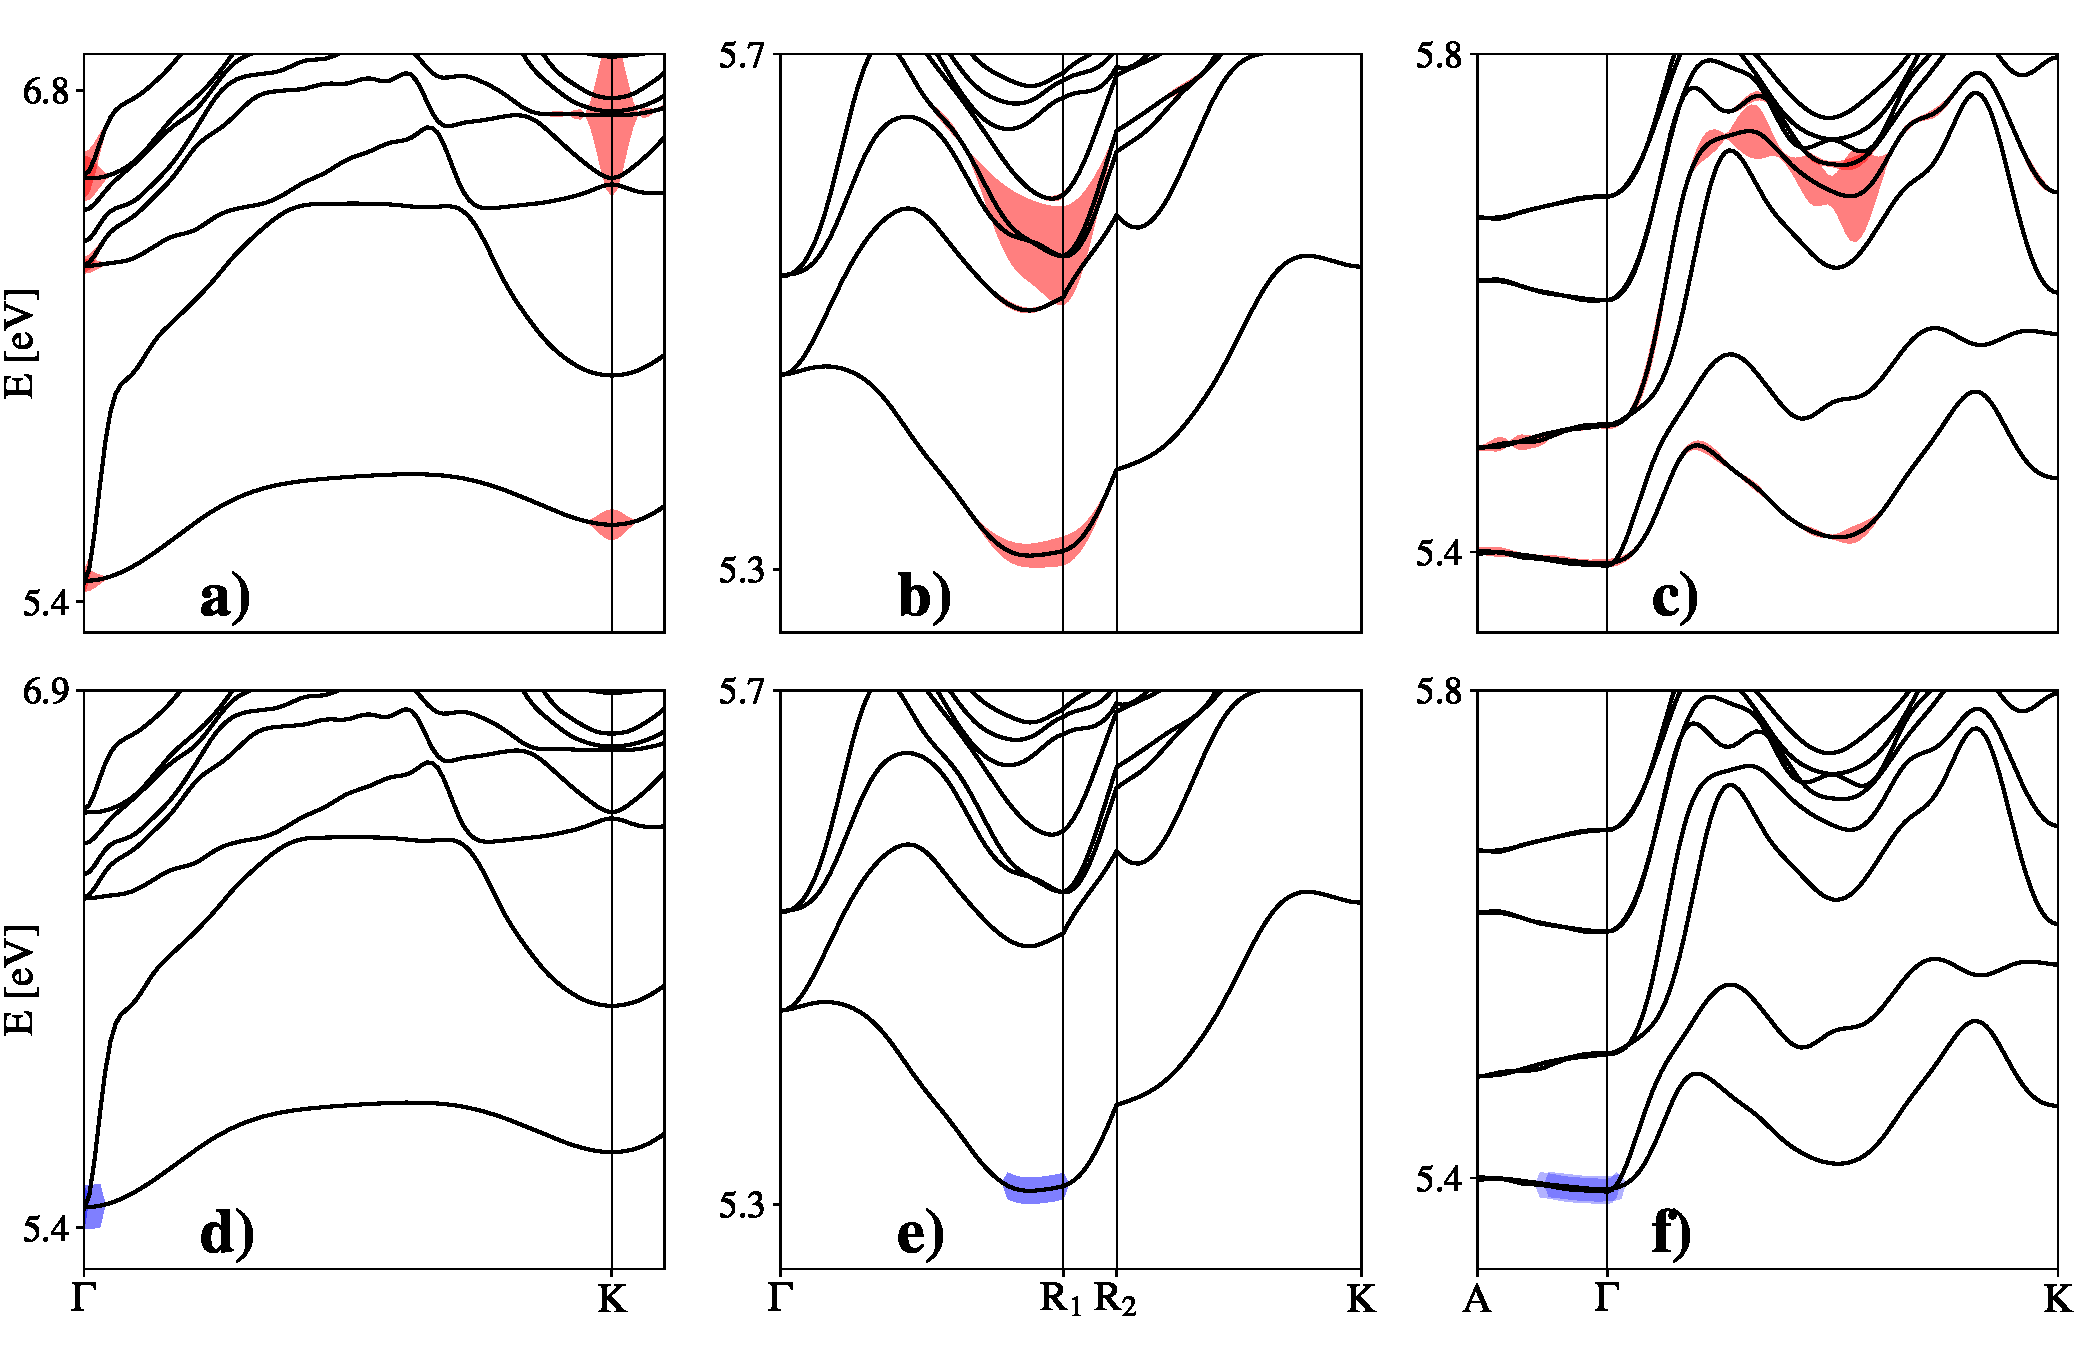
\includegraphics[width=0.9\textwidth]{all_occupations.pdf}
	\caption{Comparison of Boltzmann (blue areas) and quasi-Fermi (red areas) excitonic occupations for mBN, hBN and bBN. See main text for the definition of the occupation functions. The black lines are the Fourier interpolation of exciton dispersions, calculated at the G$_0$W$_0$+BSE level. \textcolor{red}{Add a BZ w/ R1 \& R2, labels to distinguish the 3 materials.}}
	\label{fig:all_occup}
\end{figure}

The final expression for luminescence intensity Eq. \eqref{eq:I_PL} is to be compared with the one obtained with the finite difference method in Chapter 2, Eq. \eqref{eq:strain_vRS_PL}. Unlike the previous method where only the indirect transitions were included, in the present formula we have both the term coming from direct transitions and the term related to phonon satellites. The major theoretical advance here is that the renormalization factor from Eq. \eqref{eq:renorm_fact} allows to compare the relative intensities of the direct and the satellite peaks. Besides, the satellite energies include the addition or removal of the phonon frequency that arises from the dynamical correction in second order perturbation theory. In the derivation of the dielectric function from finite difference, the phonon frequencies were added \textit{ad hoc} because the electron-phonon corrections were static.

A difference on the numerical side is that the internal sum in Eq. \eqref{eq:I_PL} runs over all phonon modes, all exciton and all $\qq$ points, which allows to accurately include the large excitonic density of states for phonon-assisted transitions, due to the low exciton dispersion common to most of BN crystals. \textcolor{green}{I could put the phonon-assisted DOS.} Moreover, our implementation allows to use the crystal symmetries for the calculation of the \acrshort{BSE} and of the exciton-phonon matrix elements. Thanks to this we can perform the whole workflow of \textit{ab initio} calculations in the unit cell, which is also an improvement from the previous method. 

%
\section{Benchmark on bulk hBN and results for mBN}

\subsection{Exciton-phonon matrix elements resolved in momentum}
We can plot the calculated matrix elements over the \acrlong{BZ} thanks to $\qq$-dependence in Eq. \eqref{eq:Gkkp}. For the bulk hBN, we plot in Fig. \ref{fig:Gkkp_plot_hBN} the exciton-phonon coupling modulus for the lowest-lying finite-momentum excitons $\beta=1$ and $\beta=2$ scattered into the bright excitons $\lambda=3$ and $\lambda=4$ that are degenerate at $\Gamma$, for all phonon modes. We sum the excitons two by two because they are degenerate at $\Gamma$ and other points in the \acrshort{BZ}. We average over the $\qq_z$ points belonging to discrete planes orthogonal to the $\Gamma A$ line in order to have a two-dimensional plot. The quantity we plot is : 
\begin{equation}
    \frac{1}{N_{q_z}N_\mu}\sum_{\mu,q_z} |\mathcal{G}_{3+4,1+2}(\qq_\parallel)|
\end{equation}
We also plot the same quantity but keeping only ZA and ZO phonon modes in the sum. 
\begin{figure}[H]%
	\vspace{0.2cm}
	\setcapindent{2em}
	\centering
    \subfloat[All phonon modes.]{\label{Gkkp_plot_hBN:all_phonons} 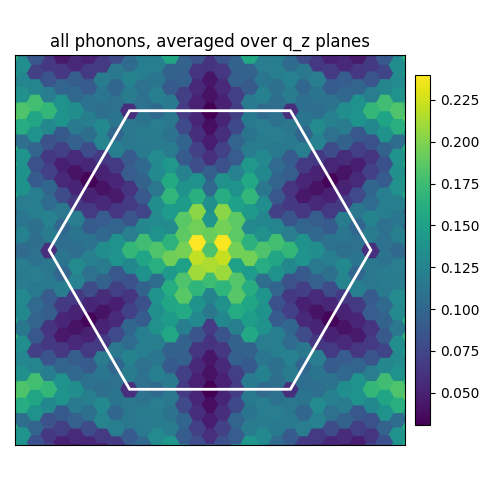
\includegraphics[width=0.45\textwidth]{hBN_all_phonons_all_planes.png}} \qquad 
    \subfloat[ZA+ZO modes only.]{\label{Gkkp_plot_hBN:z_only} 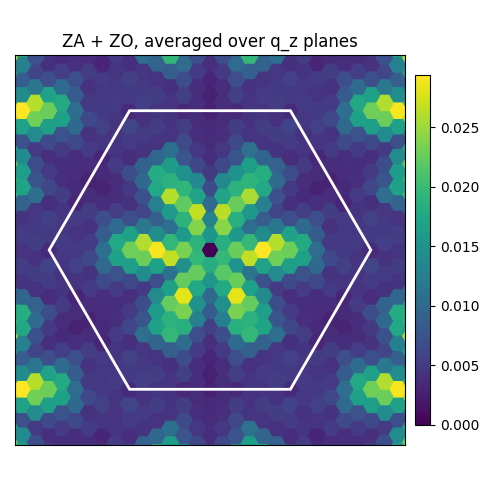
\includegraphics[width=0.45\textwidth]{hBN_z_only_all_planes.png}}%
    \caption{Magnitude of the coupling between the finite-momentum excitons and the lowest-lying bright excitons in Bernal BN. Color bar is the modulus of $\mathcal{G}(\qq)$ in eV, for a 18$\times$18 $\qq$-points grid. \textcolor{red}{add label for colorbar}}
	\label{fig:Gkkp_plot_hBN}
\end{figure}
It is the probability that the excitons $\beta=1$ and $\beta=2$ are scattered into the zero-momentum excitons $\lambda=3$ and $\lambda=4$ by all phonon modes with the corresponding momentum. The information we can extract from this plot is that the coupling has the same symmetry as the crystal, where the 6-fold rotation is clearly visible. From the panel \ref{Gkkp_plot_hBN:all_phonons}, we see that the scattering is maximal with excitons close to the $\Gamma A$ line. From the second panel \ref{Gkkp_plot_hBN:z_only}, we see that the ZA and ZO modes couple more with the minimum excitons on the $\Gamma K$ lines. This coupling contributes to about ten percent of the sum of all modes, as can be seen with the color bars.  

For the monolayer BN, we plot a similar quantity in Fig. \ref{fig:mBN_Gkkp}, except there is no need of averaging over planes since the \acrshort{BZ} is two-dimensional. We plot the scattering of finite-momentum excitons $\beta=1$ and $\beta=2$ 
into the two degenerate bright excitons $\lambda = 1$ and $\lambda = 2$ at $\Gamma$ (where the $\beta$ and $\lambda$ indices coincide).
\begin{figure}[H]
	\vspace{0.2cm}
	\setcapindent{2em}
	\centering
	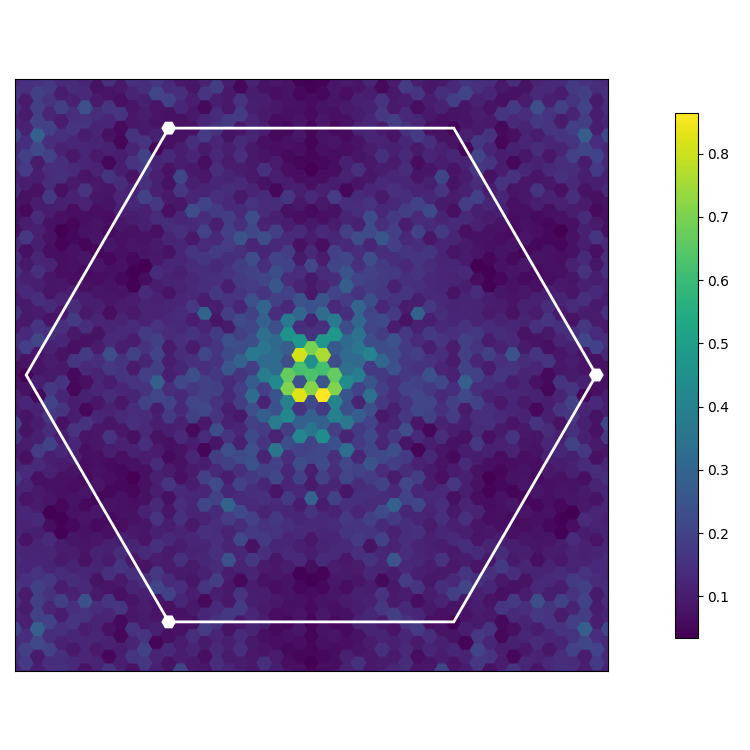
\includegraphics[width=0.55\textwidth]{mBN_Gkkp.png}
	\caption{Magnitude of the coupling between the finite-momentum excitons and the lowest-lying bright excitons in monolayer hBN. Color bar is the modulus of $\mathcal{G}(\qq)$ in eV for a $\qq$-points grid of 36$\times$36 grid. \textcolor{red}{add label for colorbar}} 
	\label{fig:mBN_Gkkp}
\end{figure}
Here the situation is different since most of the coupling happens around $\Gamma$ and is about 4 times stronger than in the bulk materials. \textcolor{red}{Do we know why it is stronger in the monolayer ?} The 6-fold hexagonal pattern can still be distinguished with lower coupling strength. This result is a first hint that in \acrshort{mBN}, it is less likely to see phonon-satellites coming from the scattering of an exciton at the \acrshort{BZ} edge than at the center.   

\subsection{Luminescence spectra}
\subsubsection{Benchmark on bulk hBN}
We now put to the test our method by calculating the luminescence spectra of bulk hBN which will serve as a benchmark. Indeed we can compare it to our finite difference method as well as existing calculations in the literature and most importantly to experiments. 
\begin{figure}[b]%
	\vspace{0.2cm}
	\setcapindent{2em}
	\centering
    \subfloat[Comparison of finite-difference and \textit{ab initio} methods.]{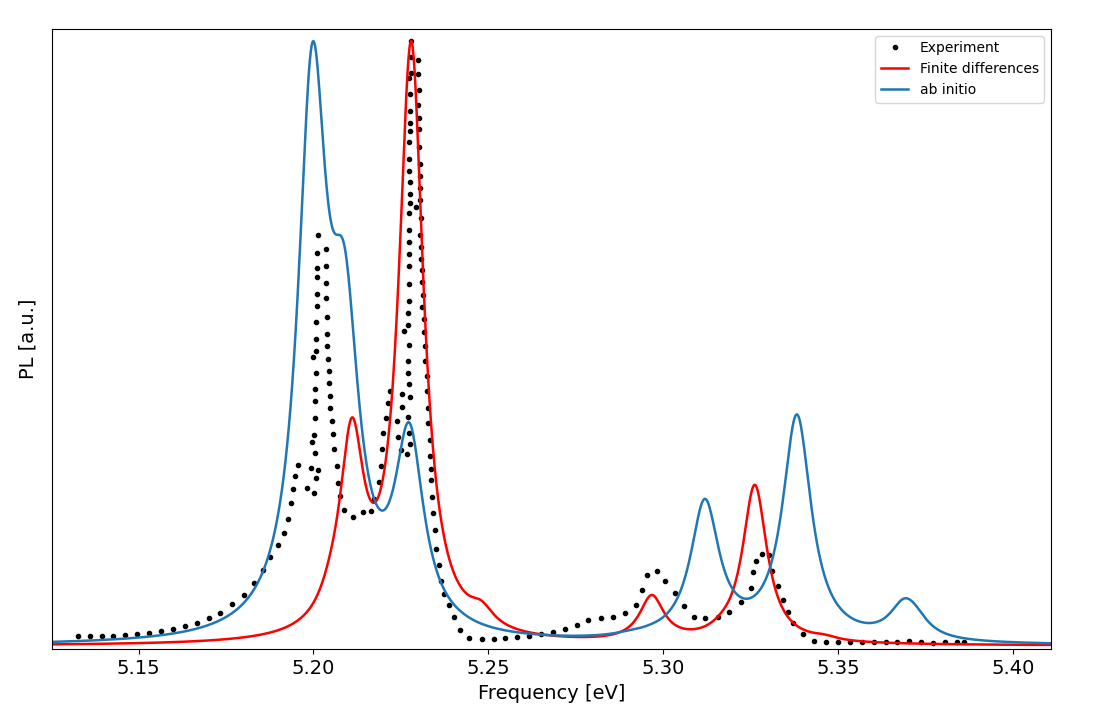
\includegraphics[width=0.45\textwidth]{comparison_pl.png}} \label{comparison_fdd} \qquad 
    \subfloat[Comparison of our \textit{ab initio} method and the one of Chen \textit{et al.}]{\label{comparison_ai} 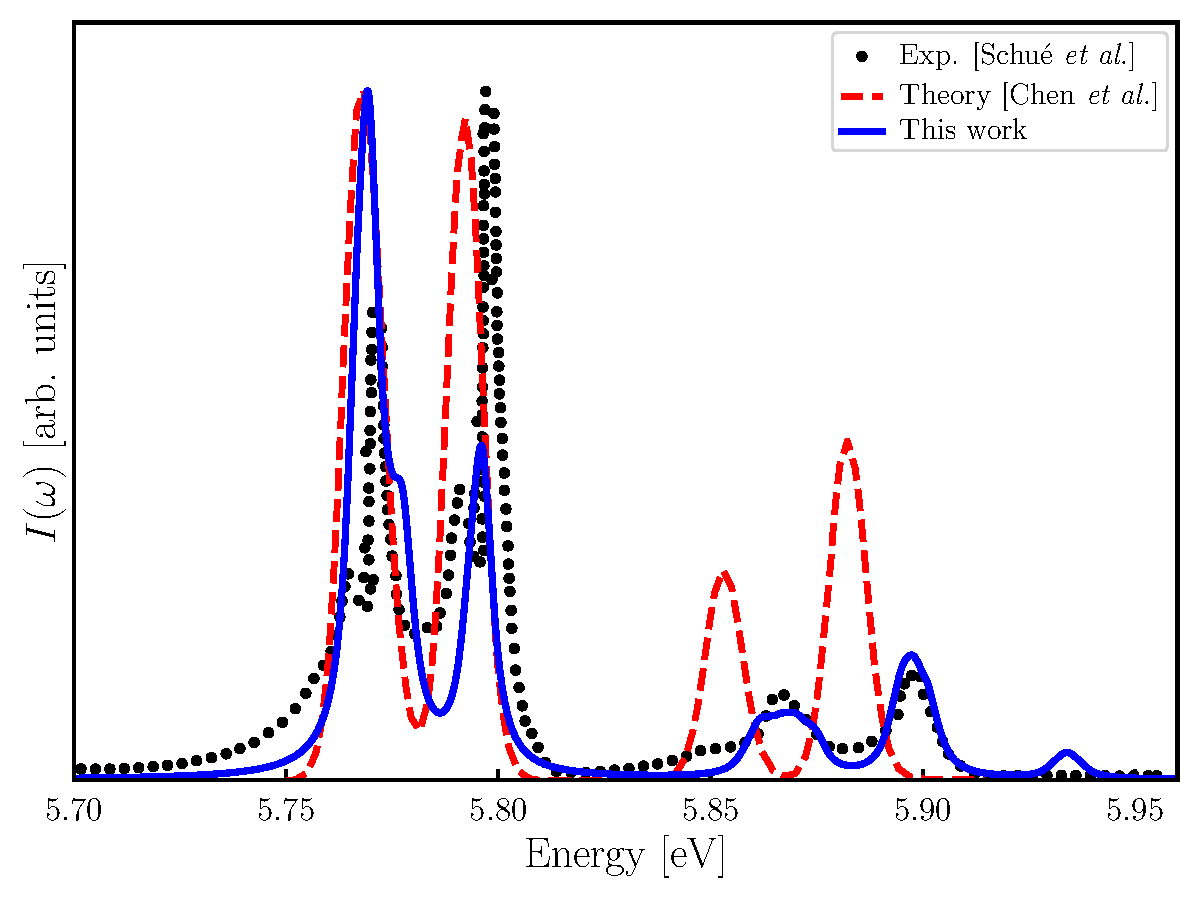
\includegraphics[width=0.45\textwidth]{hbn_pl_bulk.pdf}}%
    \caption{Comparisons of the luminescence spectrum obtained with our \textit{ab initio} method (blue line) and the finite difference method (green line) on the left panel. On the right, we compare it to the result of Ref. \cite{chen2020exciton} (red dashed line). In both panels, the experimental data (black dots) comes from Ref. \cite{schue2019bright}.}
	\label{fig:hBN_PL_comparison}
\end{figure}
In the left panel of Fig. \ref{fig:hBN_PL_comparison}, we plot the luminescence spectra obtained with the exciton-phonon coupling from finite difference, as presented in Chapter 2, compared with the present \textit{ab initio} method. The peaks are given by a Dirac delta function with a finite broadening added to follow a Lorentzian shape and match the experimental peak shapes (more numerical details can be found in Appendix \ref{sec:comp_details_Chapt3}). The shape of the LA/TA phonon satellites on the high energy side of the spectrum, computed with the present \textit{ab initio} method, are broader than the single Lorentzian peaks of the finite difference method. This is a consequence of the integration on the full $\qq$-grid present in the former method and not in the latter. In addition, we used a double-grid for the exciton energies, the phonon frequencies and the electron-phonon coupling matrix elements, so that the numerical instabilities of the renormalization factor in Eq. \eqref{eq:renorm_fact} are smoothed out and the dispersions are accurately described. We verified that we obtain similar spectra when we restrict the sum on $\qq$ in Eq. \eqref{eq:I_PL} to the $\bar{q}$ points used in Chapter 2. The difference comes from the renormalization due to the denominators in the self-energy Eq. \eqref{eq:excph_SE_compact} which is missing in the finite difference formula. It should also be noted that the inclusion of phonon absorption processes does not give additional peaks in the spectrum. Indeed, the satellites due to phonon absorption have an intensity proportional to the Bose-Einstein occupation of phonons, which is low for the lattice temperature of 10 K we simulated. We have verified that these peaks appear when the lattice temperature is increased. Similarly, we have verified that higher-energy excitons become populated by the Boltzmann occupation function when we increased $T_{exc}$ and produce satellite peaks in the spectrum. 

In the right panel of Fig. \ref{fig:hBN_PL_comparison}, we also compare our result with the spectrum obtained by Chen \textit{et al.} in Ref. \cite{chen2020exciton}. As mentioned previously, the exciton-phonon matrix elements we compute are the same than in their formulation, if we do the correct change of variable to account for their different momentum transfer convention. We implemented their convention in \yambo~and verified that the spectra do not change when using one or the other. They compute the luminescence intensity differently than the van Roosbroeck--Shockley relation, this is why the spectra look different. Our spectrum reproduces correctly the position of the satellites measured in Ref. \cite{schue2019bright} (note that all spectra have been shifted to match the energy of the experimental peaks) and the intensity of the LA/TA doublet on the high energy side, which is an improvement compared to the results of Chen \textit{et al.}. However, the intensity of the LO/TO doublet on the low energy side is not well reproduced. It is in fact inverted, with the TO peak being less intense than the LO one. Since this inaccuracy in the intensity if still in the correct order of magnitude, we decided to proceed with this implementation. It has been shown very recently in Ref. \cite{zanfrognini2023distinguishing} that this effect can be corrected by solving the \acrshort{BSE} at $\Gamma$ without the long-range component of the Coulomb interaction, hence using $\bar{\chi}$ from Eq. \eqref{eq:chi_bar} instead of the full $\chi$ from Eq. \eqref{eq:chi_iL}. We can also notice that the experimental peaks have phonon overtones due to the scattering with multiple phonon,\cite{vuong2017exciton} and this is not included in our framework.

Besides, another issue in the spectrum is the presence of a low intensity peak at 5.93 eV, which appear neither in other numerical spectra, nor in experimental measurements. To investigate the origin of this peak, we can separate the contribution of each phonon mode to the spectrum. We plot said contributions in Fig. \ref{fig:hBN_split_phonons}
\begin{figure}[H]%
	\vspace{0.1cm}
	\setcapindent{2em}
	\centering
    \subfloat[]{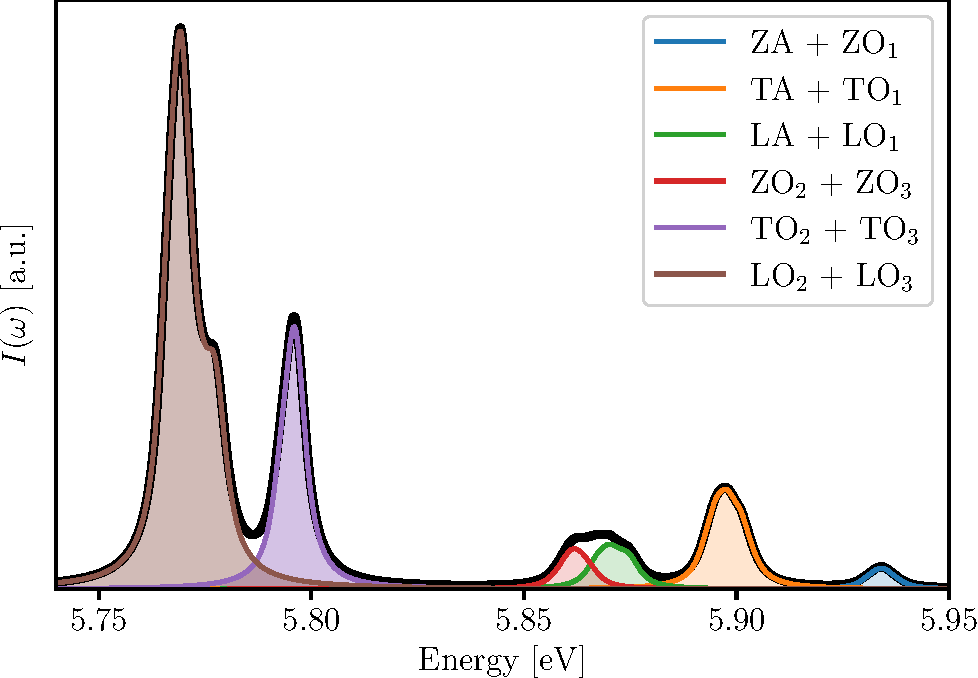
\includegraphics[width=0.6\textwidth]{hbn_pl_split_phonons.pdf}} \ 
    \subfloat[]{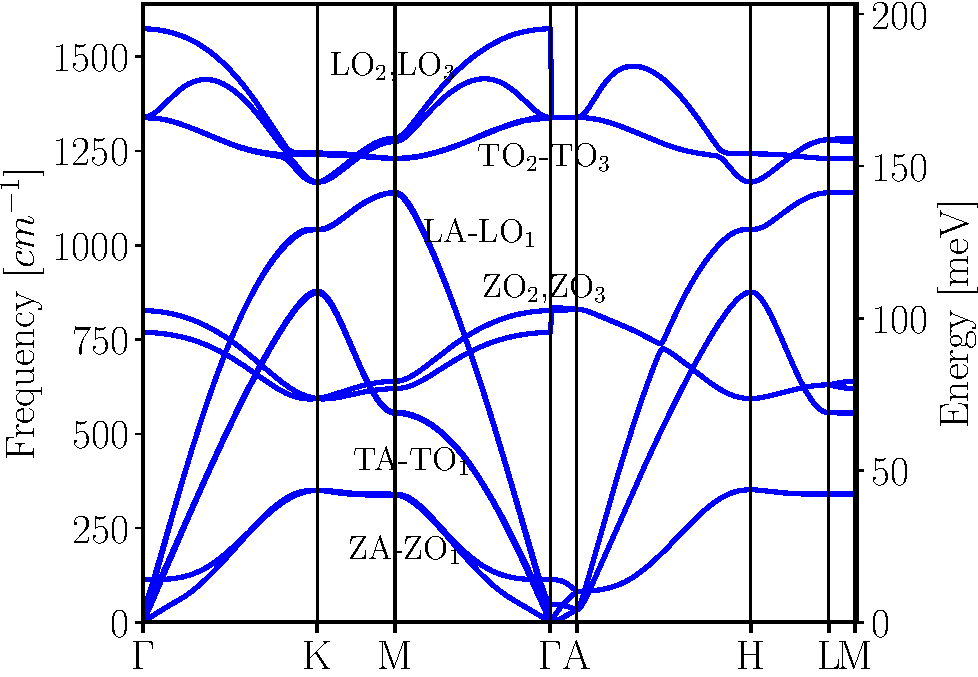
\includegraphics[width=0.39\textwidth]{hBN_phdisp.pdf}}%
    \caption{Luminescence spectrum of bulk hBN resolved with respect to the different
    phonon modes on the left panel and phonon dispersion on the right panel. \textcolor{red}{}}
	\label{fig:hBN_split_phonons}
\end{figure}
We see that the additional peaks come from scattering of excitons with ZO and ZA phonon modes. In our simulations, we set the light polarization to be in-plane. Hence optically created excitons are in-plane, and their scattering with out-of-plane phonons (namely the ZA and ZO modes) and their successive recombination is forbidden by symmetry.\cite{paleari2019exciton,cassabois2016hexagonal} If the crystal symmetries are changed, then these forbidden peaks can appear in photoluminescence. It is the case for rhombohedral BN.\cite{zanfrognini2023distinguishing} In our case, the problem arises from the definition of the exciton-phonon matrix elements in Eq. \eqref{eq:Gkkp}. The electron-phonon matrix elements and the exciton eigenvectors have different random phases that depend on the different sets of Kohn-Sham wavefunctions that were used to generate them in the first place. It is a non-trivial technical and numerical issue to account for these phases consistently.  Indeed, some \acrshort{DFPT} implementations (like \textsc{Quantum ESPRESSO}) recalculate the KS wavefunctions at $\kk+\qq$ for each $\qq$. Instead, a single set of wavefunctions is used to define the BSE matrix at any momentum $\QQ$ in the \yambo code, where the $\kk+\qq$ wavefunctions are obtained by symmetry transformations, thus imposing a specific choice of the relative phase between the wavefunctions. This difference causes a phase mismatch in the definition of the exciton-phonon matrix elements, Eq.~\eqref{eq:Gkkp}, because both the electron-phonon matrix element and the excitonic coefficients enter as full complex numbers. This is likely the reason why the magnitude of the coupling with ZA and ZO phonon modes is as large as displayed in Fig. \ref{fig:hBN_PL_comparison}.
This issue remains also if the electron-phonon matrix elements are obtained via Wannier interpolation\cite{chen2020exciton}, since the wavefunction used to construct the excitonic matrix would be different from the ones resulting via the Wannier procedure. In this case the interpolation process should be modified by fixing the wavefunction phases\cite{giustino2007wannier}. 
The phase mismatch is not present in calculations based on finite differences\cite{paleari2018excitons,lechifflart2022excitons} because in this case exciton-phonon coupling is directly calculated as a derivative of the exciton dipole matrix elements on a supercell. However, these types of calculations are restricted to a single $\qq$-vector.
In the case of hBN luminescence, we verified that the phase mismatch only gives small changes in the numerical results (by testing different sets of wavefunctions with different random phases). A possible workaround was investigated very recently in Ref. \cite{zanfrognini2023distinguishing} but it requires to write an interface with a third simulation code and most importantly to turn off all crystal symmetries, which considerably slows down all calculation and requires a lot more disk space.

Overall, our spectrum is in rather good agreement with the experimental one. Keeping in mind the issues discussed above, we turn to the study of a case where the main advantage of our method is useful : the fact that we can compare the relative intensities of direct peaks and phonon satellites.

\subsubsection{Results on mBN}
PL with 4 experiments, discussion on the absence of K satellite and size of the Gamma one

\section{effects of the substrate}
electronic gap, distortion of excitonic dispersion to simulate a change in the screening.

\section{Preliminary results on bBN}
show the distorted spectrum, which also contains the ZO peaks\\
For Bernal BN the same quantity is plotted in Fig. \ref{fig:Gkkp_plot_hBN}, the coupling is very similar for all phonon modes, but concerning the ZA and ZO modes, the matrix elements are more homogeneous and the coupling is non-zero over the whole \acrshort{BZ}, although the magnitude is slightly lower than for hBN.
\begin{figure}[H]%
	\vspace{0.2cm}
	\setcapindent{2em}
	\centering
    \subfloat[All phonon modes.]{\label{Gkkp_plot_bBN:all_phonons} 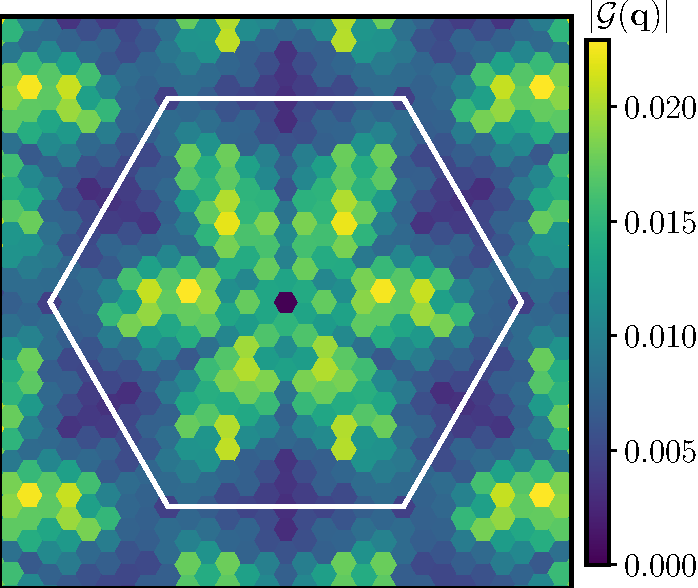
\includegraphics[width=0.45\textwidth]{bBN_Gkkp_allphonons.pdf}} \qquad 
    \subfloat[ZA+ZO modes only.]{\label{Gkkp_plot_bBN:z_only} 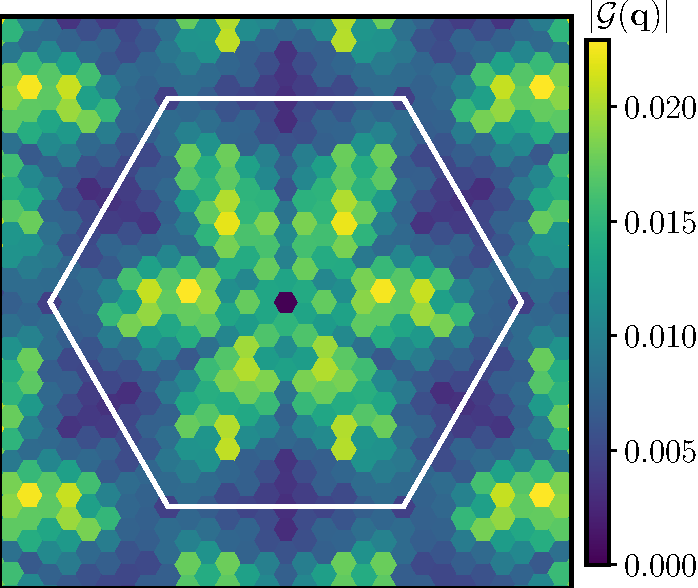
\includegraphics[width=0.45\textwidth]{bBN_Gkkp_zonly.pdf}}%
    \caption{Magnitude of the coupling between the finite-momentum excitons and the lowest-lying bright excitons in Bernal BN. Color bar is the modulus of $\mathcal{G}(\qq)$ in eV, for a 18$\times$18 $\qq$-points grid. \textcolor{red}{add label for colorbar}}
	\label{fig:Gkkp_plot_bBN}
\end{figure}


\section{Conclusion of the chapter}
need to solve the phase problem 
natural extension to cumulant for multi phonons

